\subsection{Android Application Package (APK)} \label{subsection:foundation-android-package}
\begin{itemize}
    \item test
\end{itemize}
Android applications are distributed and installed using the \gls{apk} file format.
They can either be obtained from an application store, like Google Play, or downloaded and installed, manually or by using \gls{adb}, from any other source.

The \gls{apk} format is based on the ZIP file archive format and contains the code and resources of the application.
The build process of \gls{apk} contains several steps which are visualized in figure~\ref{fig:apk}.
\newline
\begin{figure}[h]
    \centering
    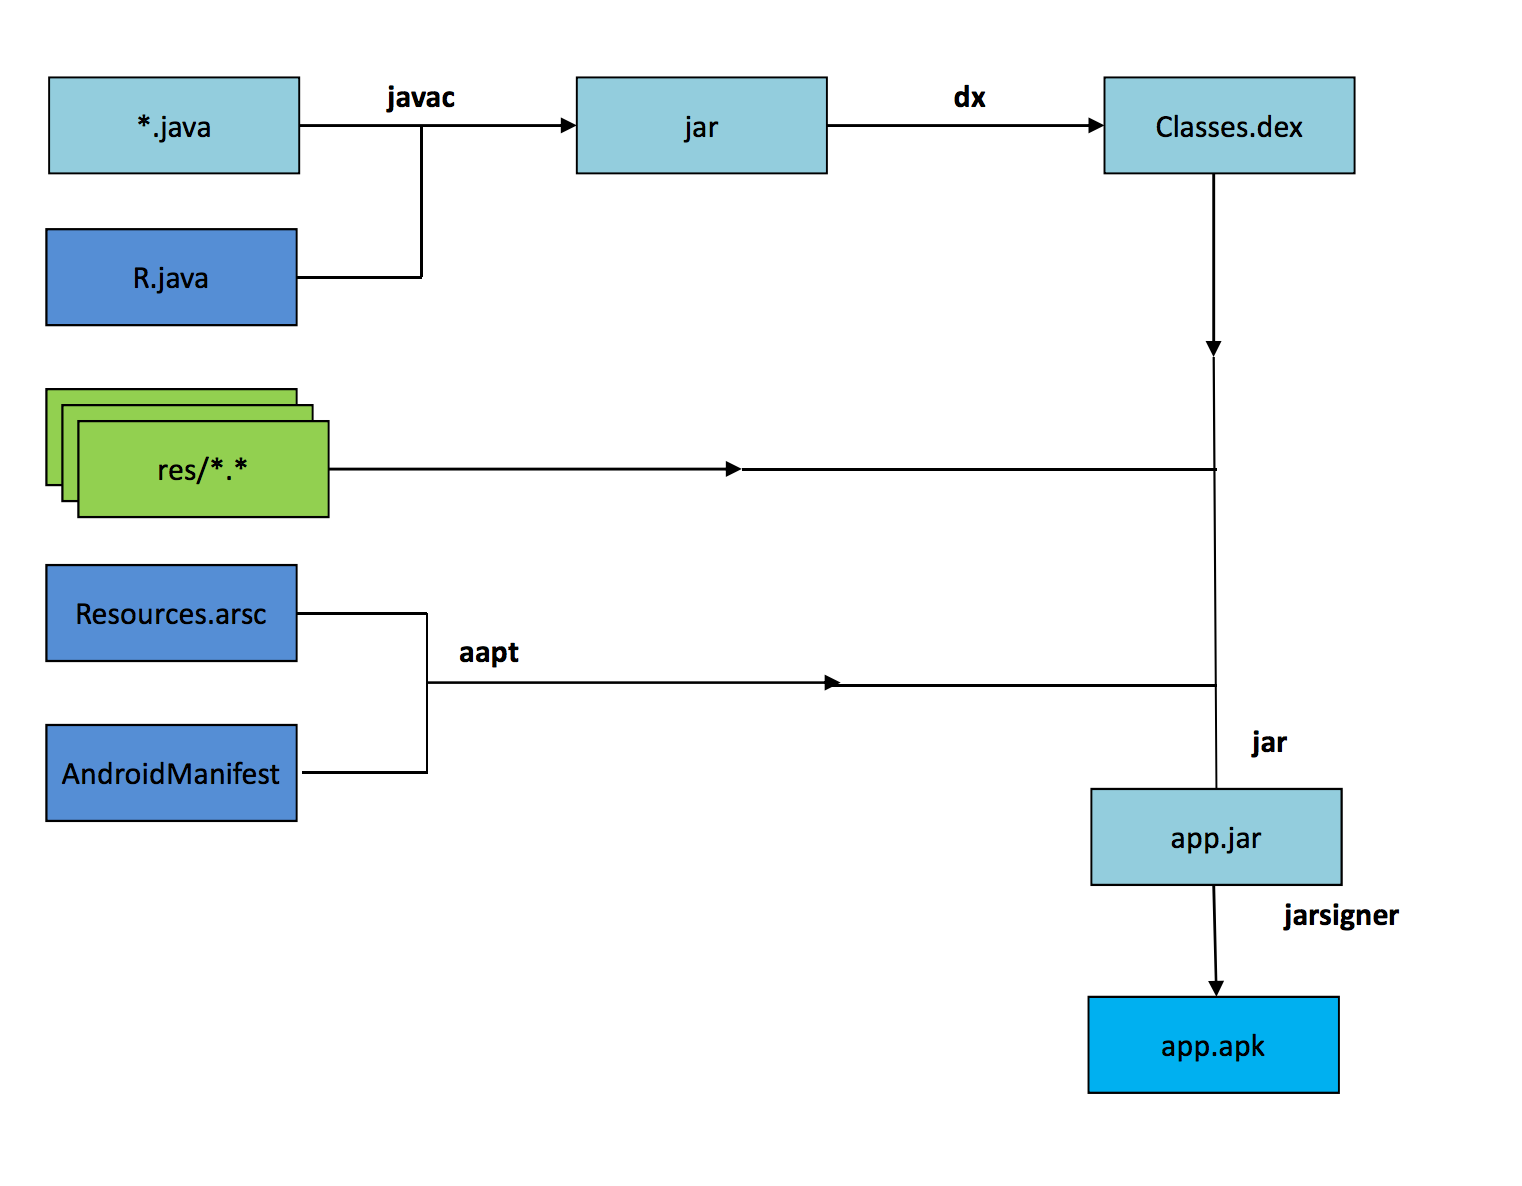
\includegraphics[width=0.8\textwidth]{data/apk.png}
    \caption{\gls{apk} build process \cite{andevconDalvikART}}
    \label{fig:apk}
\end{figure}
Since Android applications are usually written in Java, the start is similar to the Java program build process.
The Java source code is compiled into \gls{classg} file by the Java Compiler javac.
Each \gls{classg} files contains the Java bytecode of the corresponding Java class.
As an additional option in the compilation a Java obfuscator can be applied (see section~\ref{subsection:counter-improve-obfuscation}).
In the end of the Java compilation process, the .class files are packed into a \gls{jar} file.
\newline
Since Android is using the \gls{dvm}, which will be described in section~\ref{subsection:android-dalvik}, the Java bytecode has to be converted to Dalvik bytecode.
The Android \gls{sdk} includes the tool dx which is used to convert \gls{classg} files to a single classes.dex file containing all classes.
The \gls{dex} format will be described in \ref{subsection:android-dex}.
Additional obfuscation techniques can be applied to protect the \gls{dex} code \cite{dexProtector}.
\newline
Now the three main parts of the \gls{apk} are available:
\begin{itemize}
\item classes.dex, contains the bytecode
\item resources files (\textit{res/*.*}), contains static content like images, layouts and native code
\item resources.arsc and AndroidManifest.xml, contain compiled resources respectively essential information like needed permissions
\end{itemize}
These parts are combined by the ApkBuilder into one archive file.
\newline
Finally, jarsigner adds the developer’s signature to this package which does not improve security of the application itself, but identifies the developer and thus supports updates.
\newline
\newline
The structure of a final application file has at least the following content seen in figure~\ref{fig:apkfolder}.
\begin{figure}[h]
    \centering
    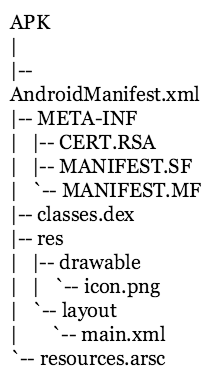
\includegraphics[width=0.5\textwidth]{data/apkfolder.png}
    \caption{\gls{apk} folder structure}
    \label{fig:apkfolder}
\end{figure}
The AndroidManfiest.xml and the classes.dex, which have been covered already.
The META-INF folder, which is inherited from Java and used to store package and extension configuration data and other \cite{metaJava}.
While the static resources, like drawables and layouts, are in the res folder, the resources.arsc contains the compiled resources.
In case the application implements native code, it is stored in the libs folder, split by the different processor types, like armeabi-v7a for ARM or x86 for Intel processors. \cite{kovachevaMaster} \cite{ehringerDalvik}
